\documentclass[tikz,border=3pt]{standalone}
\usepackage[utf8]{inputenc}
\usepackage[T1]{fontenc}
\usepackage{libertinus}
\usepackage{amsmath,amssymb}
\usetikzlibrary{arrows.meta,calc,patterns,decorations.pathmorphing,decorations.markings,decorations.pathreplacing,bending}
\definecolor{UGblue}{RGB}{0,51,102}
\newcommand{\dbar}{\mathchar'26\mkern-12mu d}
\tikzset{
  >=Stealth,
  every node/.style={font=\small},
  caja/.style={draw,line width=0.9pt},
  pared/.style={draw,line width=1.6pt},
  ejes/.style={->,line width=0.8pt},
  adia/.style={draw,pattern=north east lines,pattern color=black!70,line width=0.5pt},
  gas/.style={fill=UGblue!8},
  punto/.style={fill,circle,inner sep=1.3pt},
  onda/.style={decorate,decoration={snake,amplitude=1.1pt,segment length=5pt,post length=3pt,pre length=0pt}},
}
\begin{document}
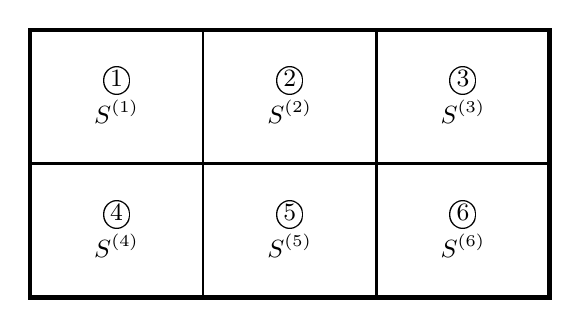
\begin{tikzpicture}
  \draw[pared] (0,0) rectangle (6.6,3.4);
  \draw[caja] (2.2,0) -- (2.2,3.4);
  \draw[caja] (4.4,0) -- (4.4,3.4);
  \draw[caja] (0,1.7) -- (6.6,1.7);
  \foreach \i/\x/\y in {1/1.1/2.55,2/3.3/2.55,3/5.5/2.55,4/1.1/0.85,5/3.3/0.85,6/5.5/0.85} {
    \node[align=center] at (\x,\y) {\normalsize \textcircled{\small\i}\\[2pt] $S^{(\i)}$};
  }
\end{tikzpicture}
\end{document}
